\documentclass[aspectratio=169]{beamer}

\usepackage[utf8]{inputenc}
\usepackage[T5]{fontenc}
\usepackage[english]{babel}
\usepackage{graphicx}
\usepackage{amsmath}
\usepackage{amssymb}
\usepackage{hyperref}
\usepackage{caption}
\usepackage{tikz}
\usetikzlibrary{positioning}

\usetheme{Madrid}
\usecolortheme{default}
\setbeamertemplate{footline}[frame number]
\setbeamertemplate{navigation symbols}{}

\title[Sign Language Recognition with ST-GCN]{WORD-LEVEL SIGN LANGUAGE RECOGNITION USING SPATIAL--TEMPORAL GRAPH CONVOLUTIONAL NETWORKS (ST-GCN)}
\author[Group 24]{
    \small
    \textbf{Students:}
    Đặng Xuân Minh Hiếu (24002005),
    Mai Hoàng Đức (22001565),
    Lê Quý Công (22001550)\\
    \vspace{0.1cm}
    \textbf{Supervisor:}
    Dr. Cao Văn Chung
}
\institute[HUS]{Faculty of Mathematics, Mechanics and Informatics \\ VNU University of Science}
\date{Hanoi, 2026}

\begin{document}

\begin{frame}
    \titlepage
\end{frame}

\begin{frame}{Outline}
    \tableofcontents[hideallsubsections]
\end{frame}

% ==========================================
\section{1. Overview and Theoretical Background}
% ==========================================
\begin{frame}{Motivation and Challenges}
    \begin{itemize}
        \item \textbf{Significance:} Communication barriers faced by the deaf and hard-of-hearing community.
        \item \textbf{RGB challenges:} Background noise, viewpoint variation, and high computational cost.
        \item \textbf{Skeleton-based solution:} Noise-robust, lightweight, and geometrically stable.
    \end{itemize}
\end{frame}

\begin{frame}{Feature Extraction with the MediaPipe Tasks API}
    \begin{columns}
        \begin{column}{0.5\textwidth}
            \begin{itemize}
                \item Employs the \textbf{Pose \& Hand Landmarker}.
                \item Extracts $\mathbf{V=75}$ landmarks:
                \begin{itemize}
                    \item 33 pose landmarks.
                    \item 21 left-hand landmarks.
                    \item 21 right-hand landmarks.
                \end{itemize}
                \item Input tensor: $\mathbf{X} \in \mathbb{R}^{3 \times T \times 75}$.
            \end{itemize}
        \end{column}
        \begin{column}{0.5\textwidth}
            \begin{figure}
                \centering
                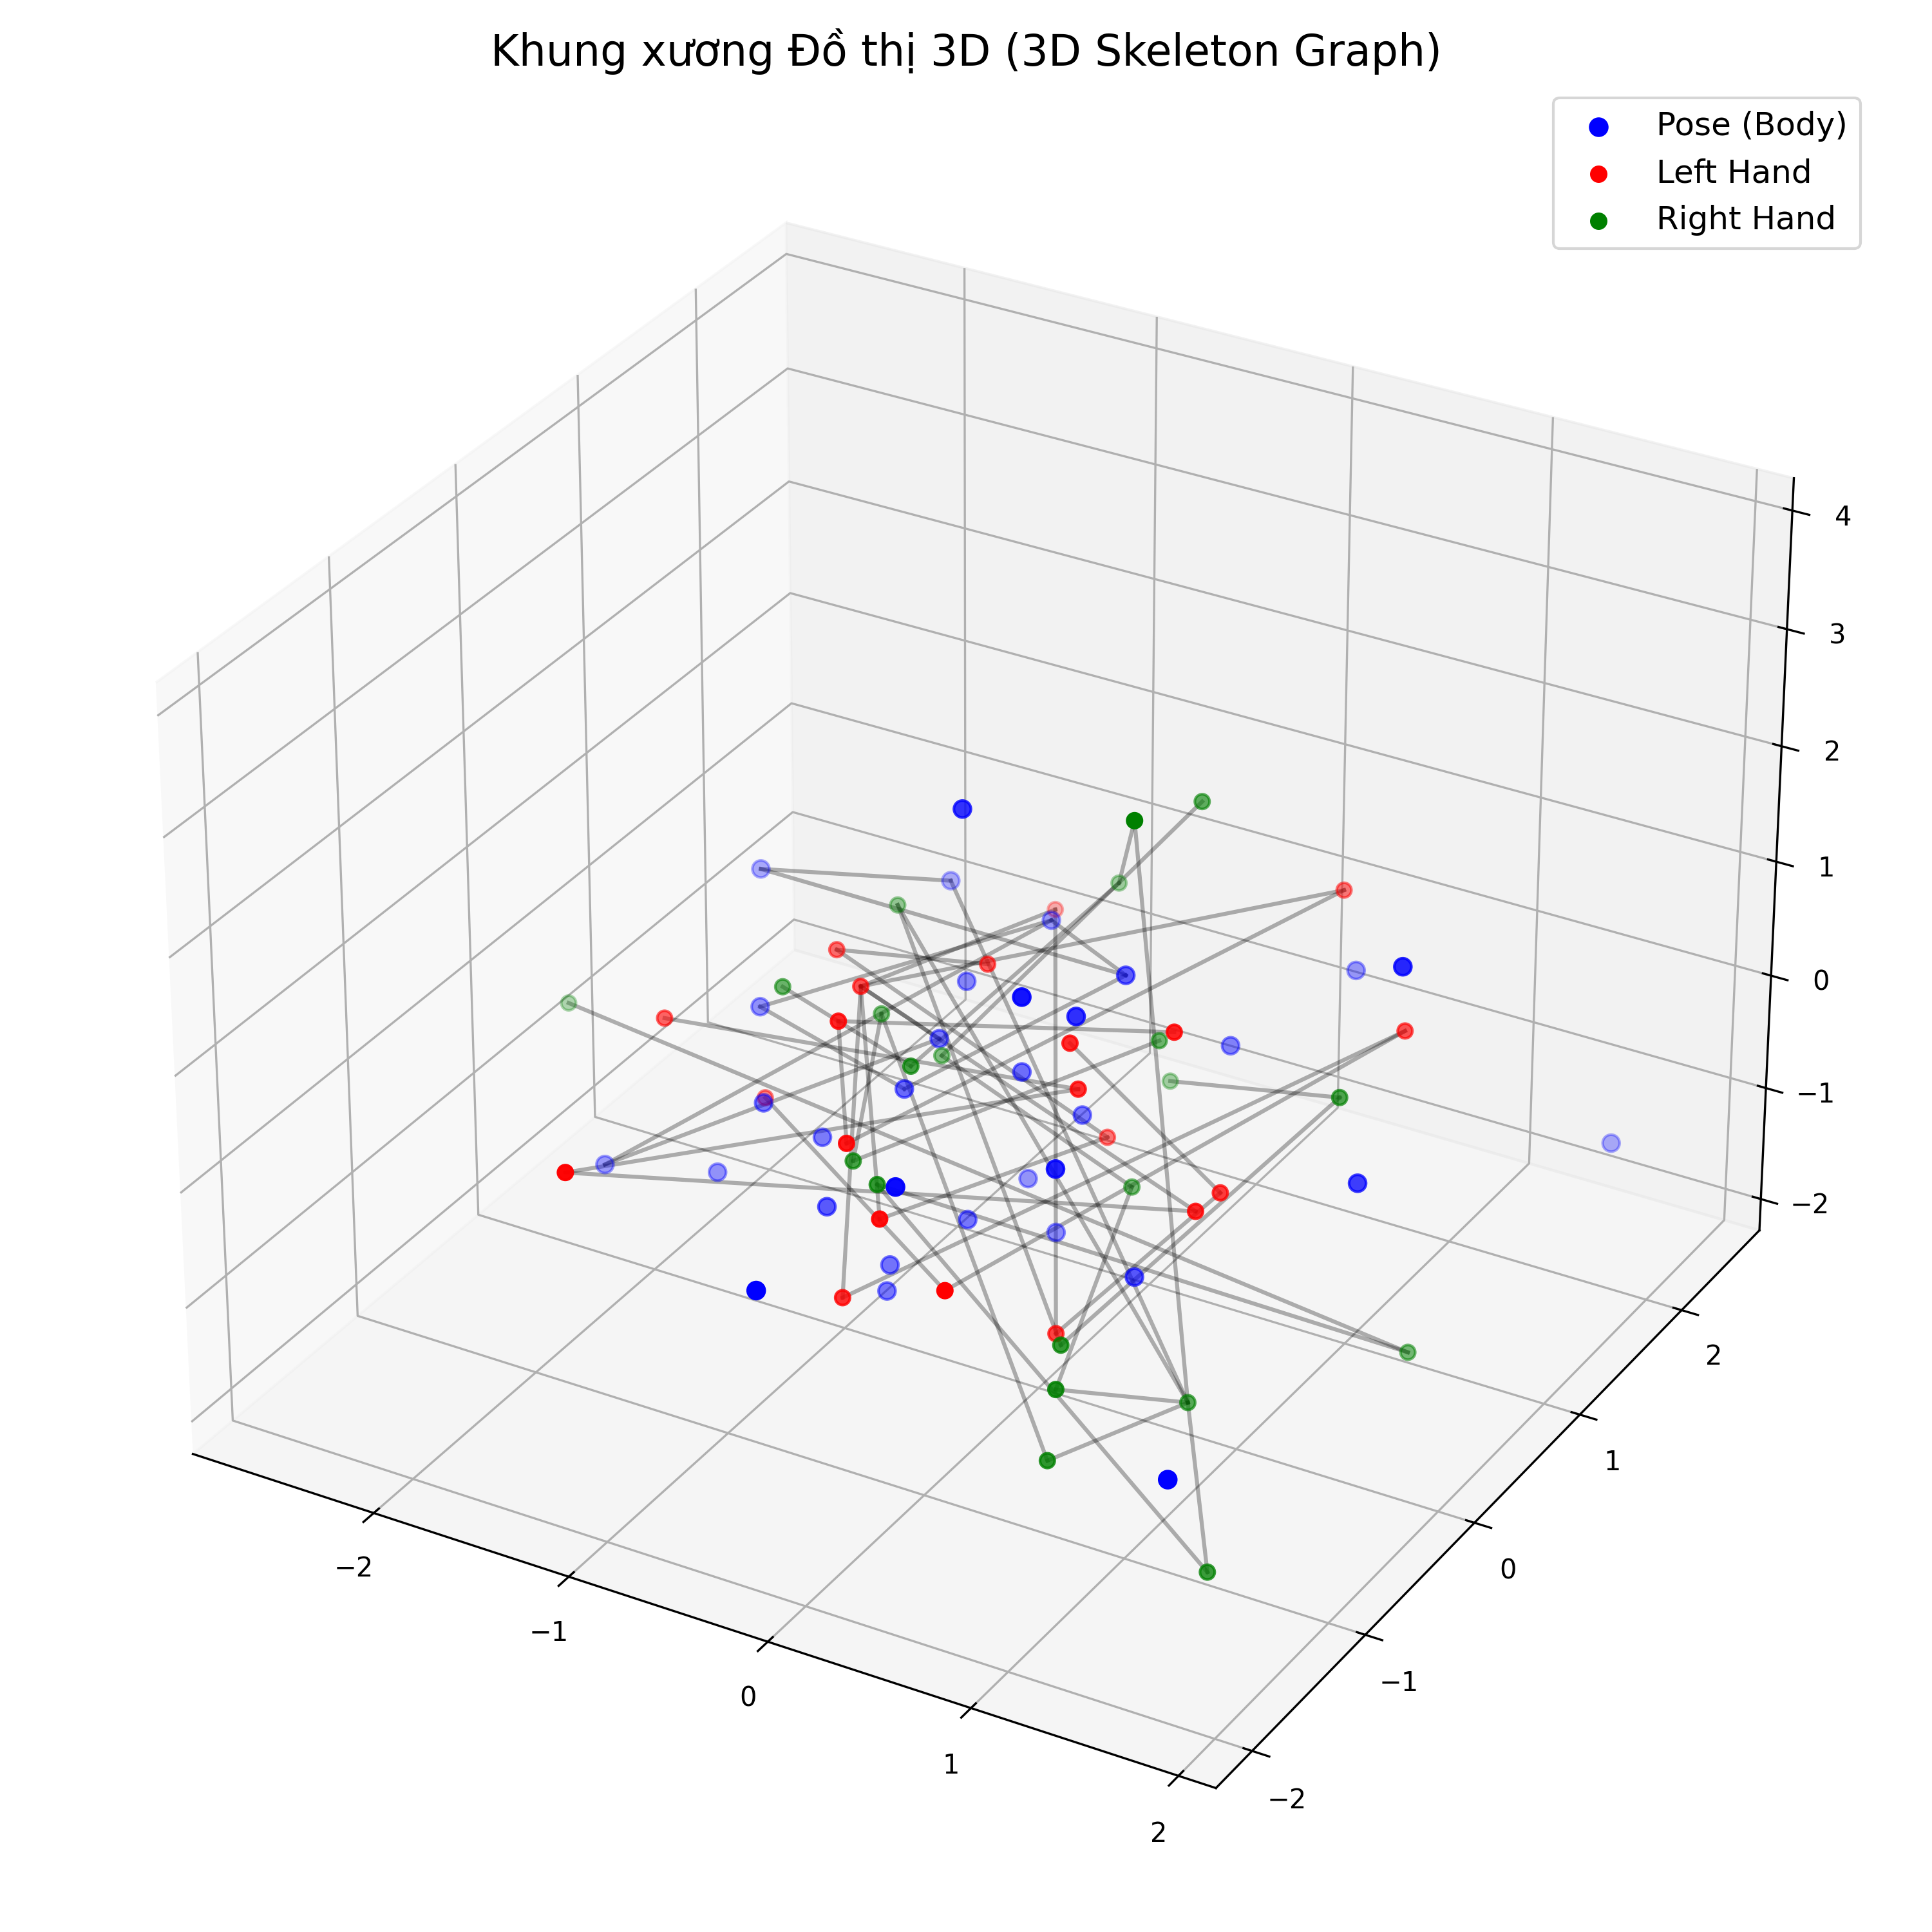
\includegraphics[height=0.6\textheight]{report/images/skeleton_3d.png}
                \caption{Skeletal connectivity structure}
            \end{figure}
        \end{column}
    \end{columns}
\end{frame}

% ==========================================
\section{2. Proposed Method and System Architecture}
% ==========================================
\begin{frame}{Analysis of the WLASL-100 Dataset}
    \begin{columns}
        \begin{column}{0.48\textwidth}
            \begin{figure}
                \centering
                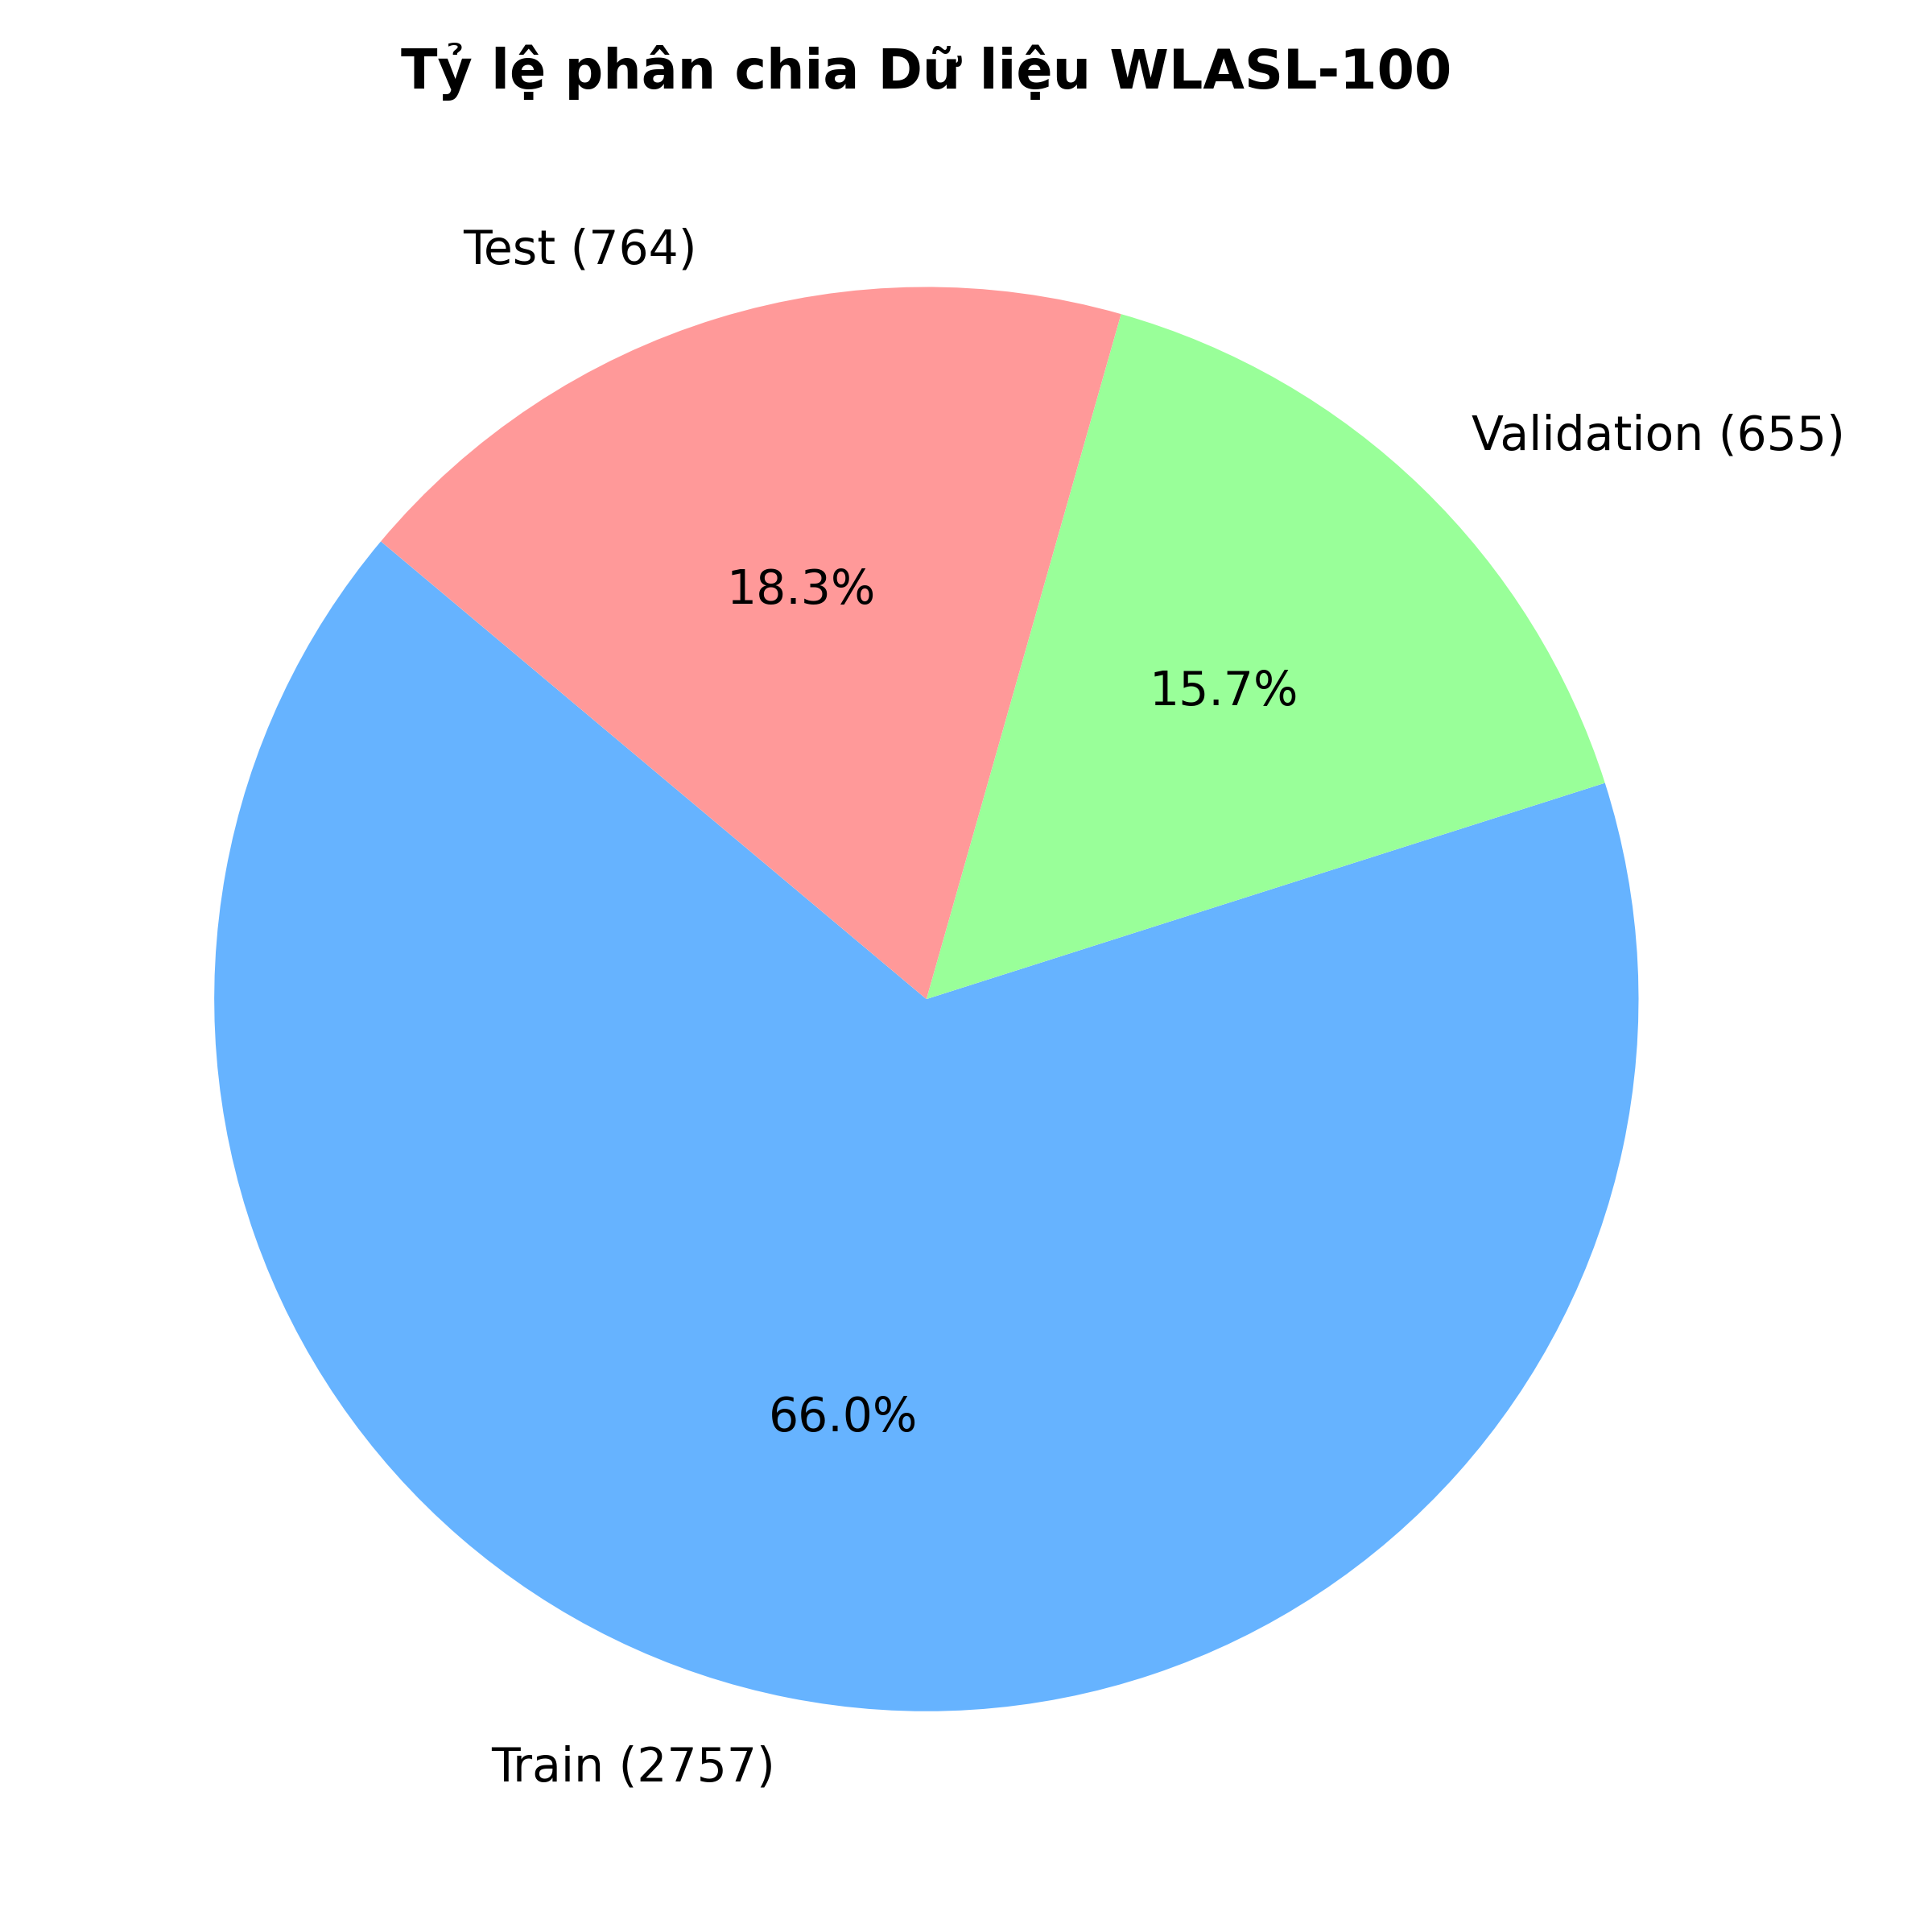
\includegraphics[width=\textwidth]{report/images/dataset_pie.png}
                \caption{Train/Val/Test split}
            \end{figure}
        \end{column}
        \begin{column}{0.48\textwidth}
            \begin{figure}
                \centering
                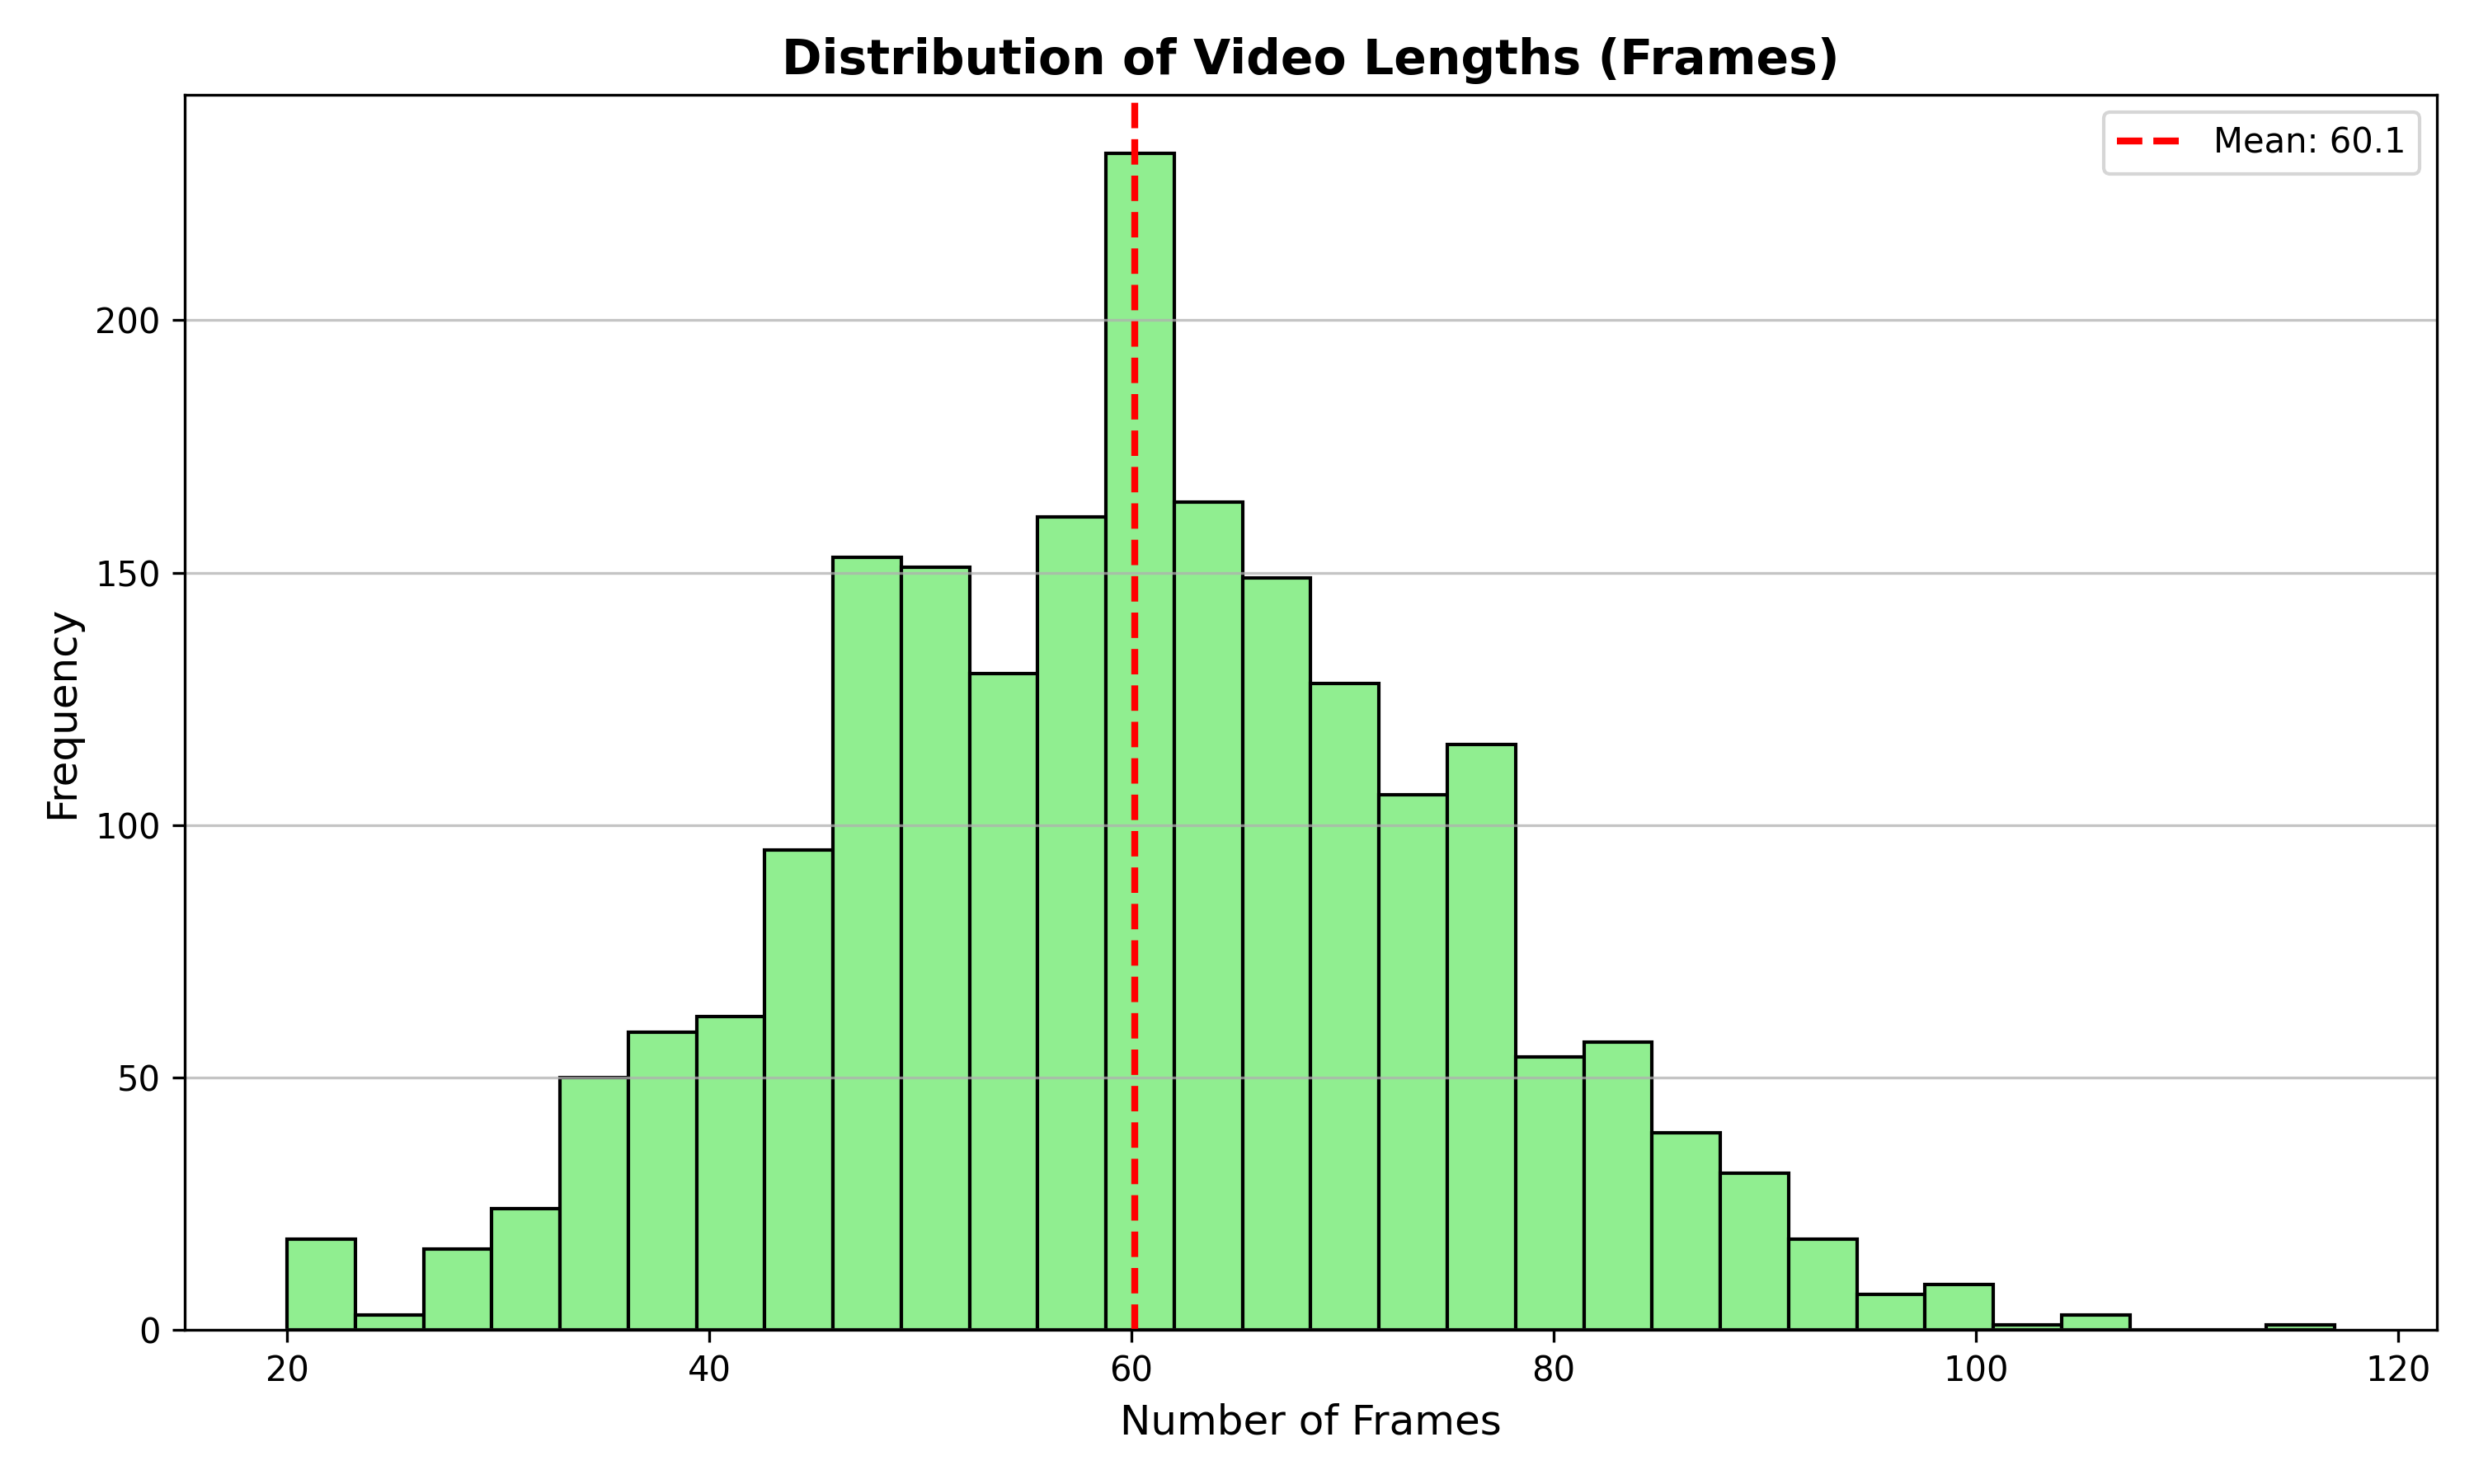
\includegraphics[width=\textwidth]{report/images/frames_histogram.png}
                \caption{Sequence-length distribution}
            \end{figure}
        \end{column}
    \end{columns}
\end{frame}

\begin{frame}{Improved ST-GCN Architecture}
    \begin{itemize}
        \item \textbf{Depth:} Scaled up to 6 ST-GCN blocks.
        \item \textbf{Adaptive graph:} A learnable, dynamic adjacency matrix.
        \item \textbf{Pipeline:}
        \begin{enumerate}
            \item Spatial GCN: learns hand shape.
            \item Temporal CNN: learns motion (kernel $=9$).
        \end{enumerate}
        \item \textbf{Techniques:} Residual connections, batch normalization, dropout.
    \end{itemize}
\end{frame}

% ==========================================
\section{3. Experiments and Results}
% ==========================================
\begin{frame}{Experimental Results}
    \begin{columns}
        \begin{column}{0.6\textwidth}
            \begin{figure}
                \centering
                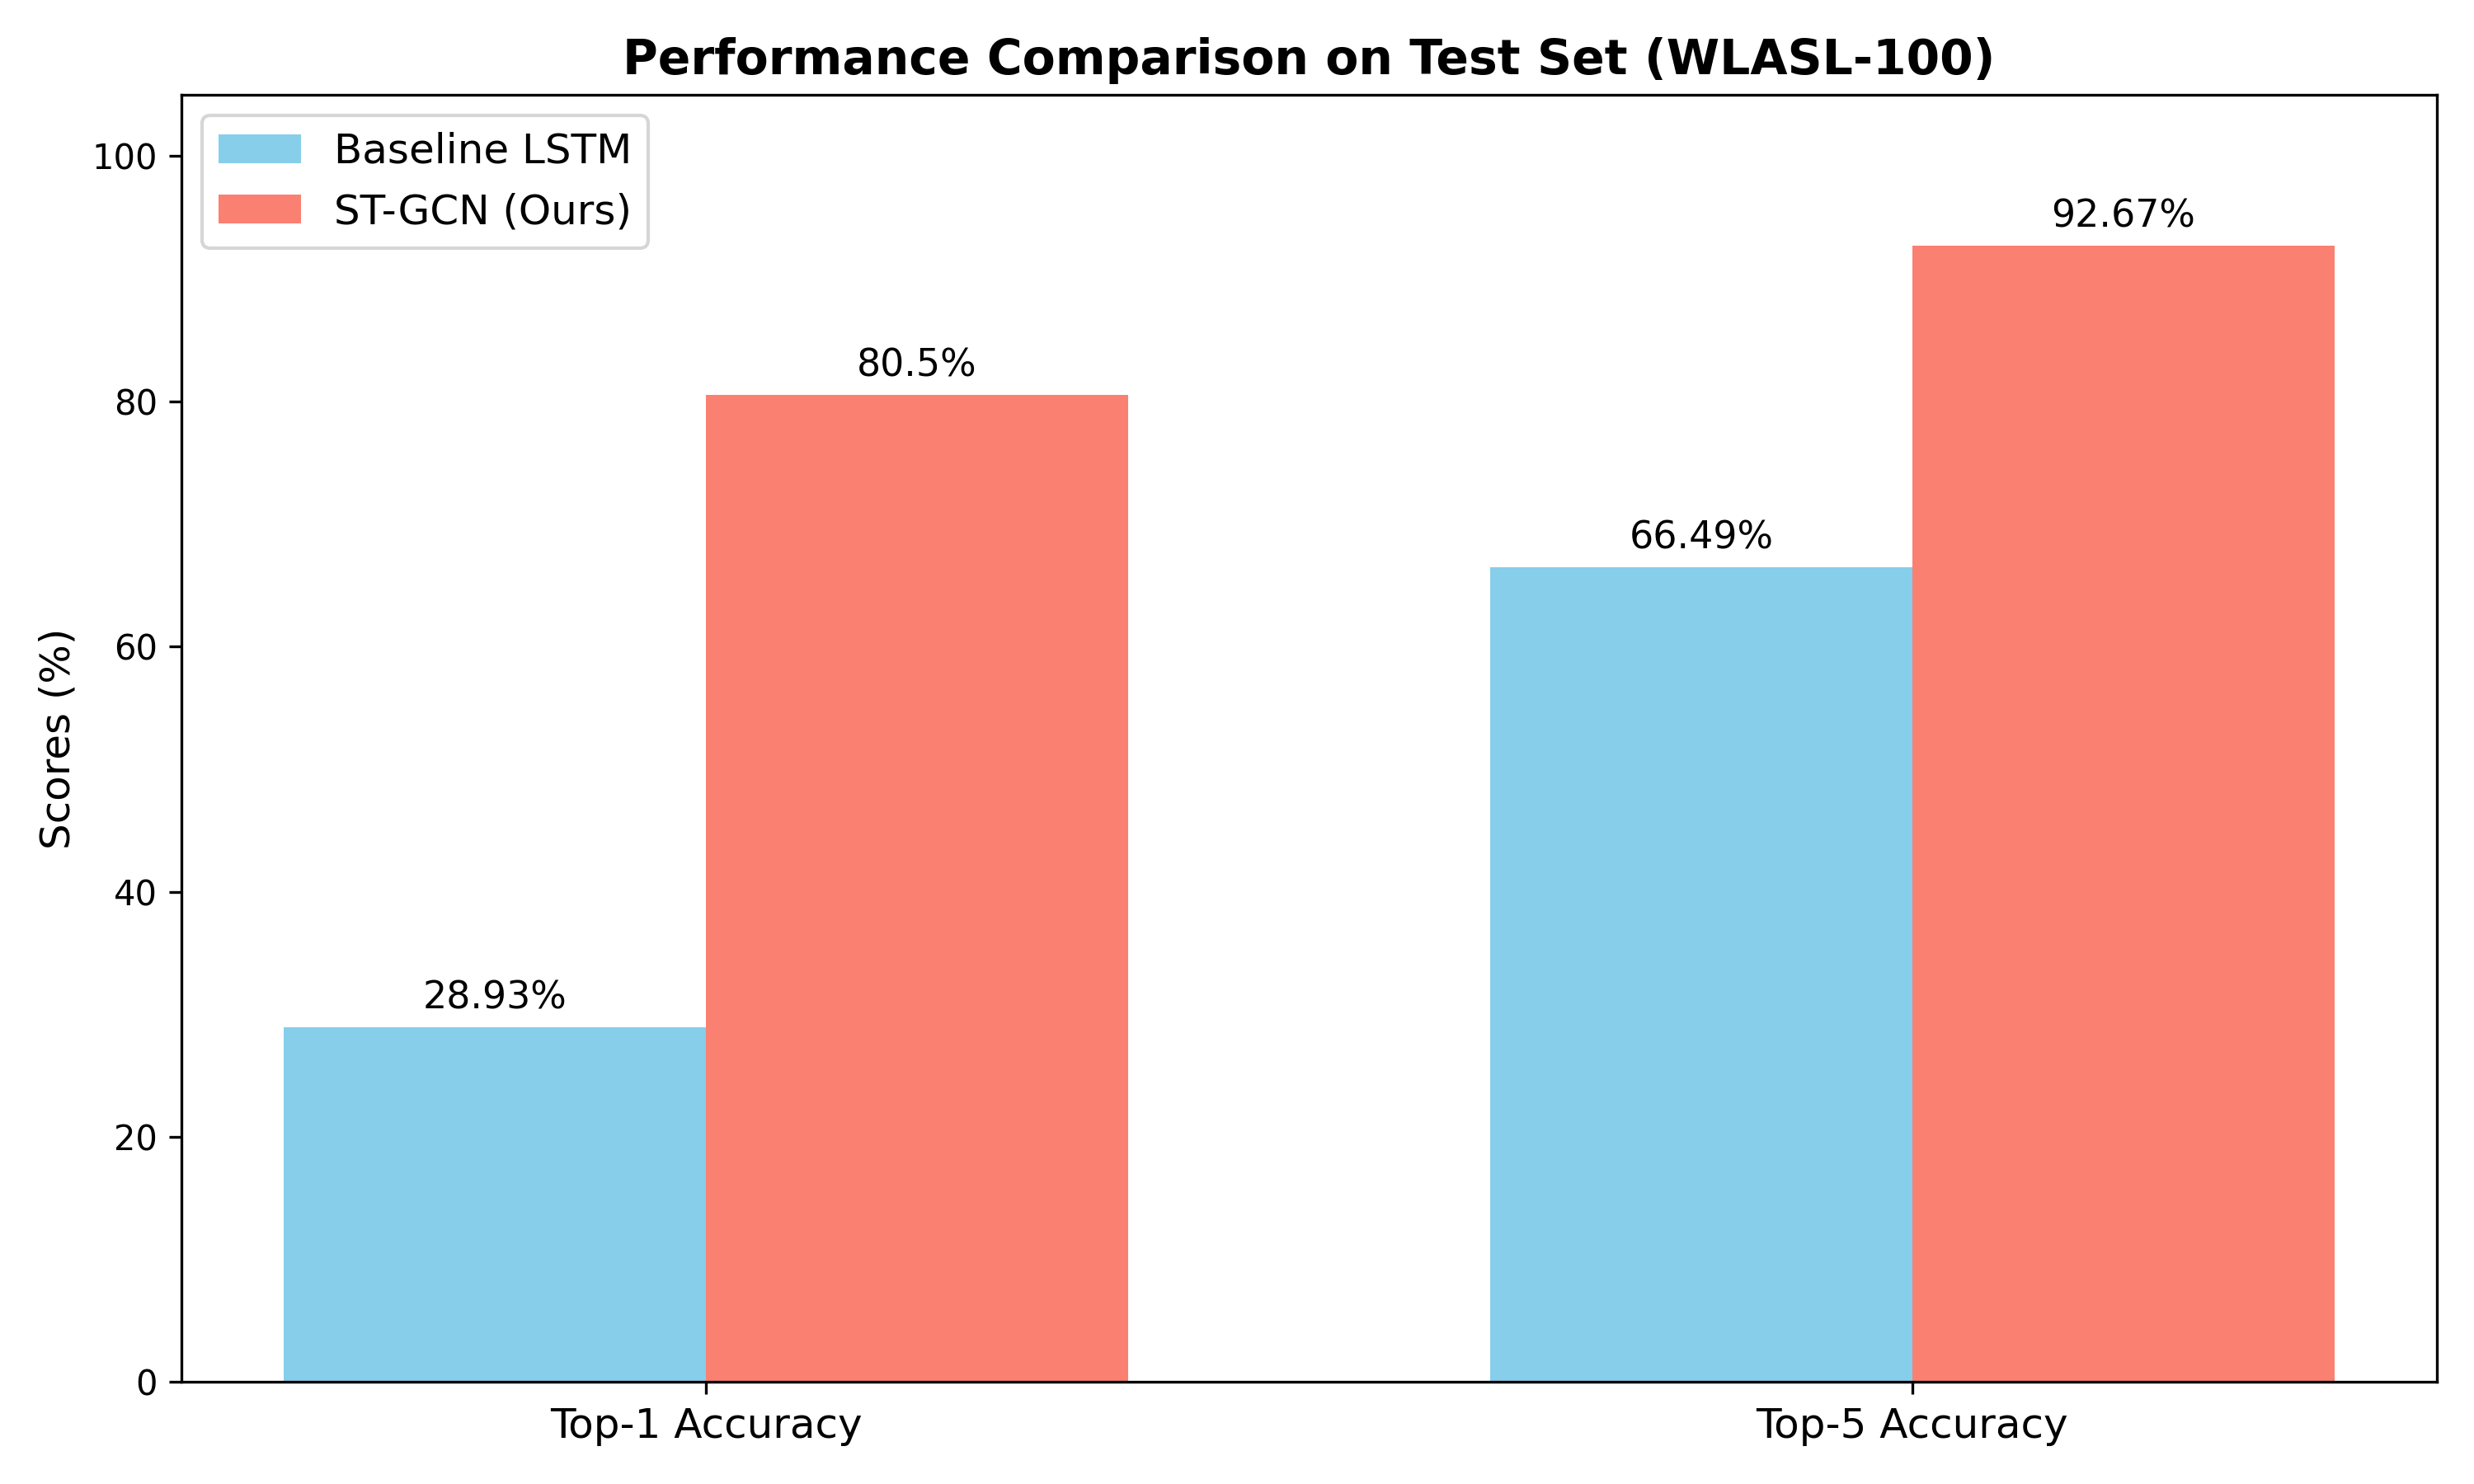
\includegraphics[width=\textwidth]{src/performance_bar_chart.png}
                \caption{Accuracy on the test set}
            \end{figure}
        \end{column}
        \begin{column}{0.35\textwidth}
            \small
            \textbf{Measured ST-GCN metrics:}
            \begin{itemize}
                \item \textbf{Top-1 accuracy:} $67.79\%$
                \item \textbf{Top-5 accuracy:} $88.0\%$
            \end{itemize}
            \vspace{0.2cm}
            \textit{The model attains stable accuracy and recognizes the 100-word vocabulary well.}
        \end{column}
    \end{columns}
\end{frame}

\begin{frame}{Confusion Matrix}
    \begin{figure}
        \centering
        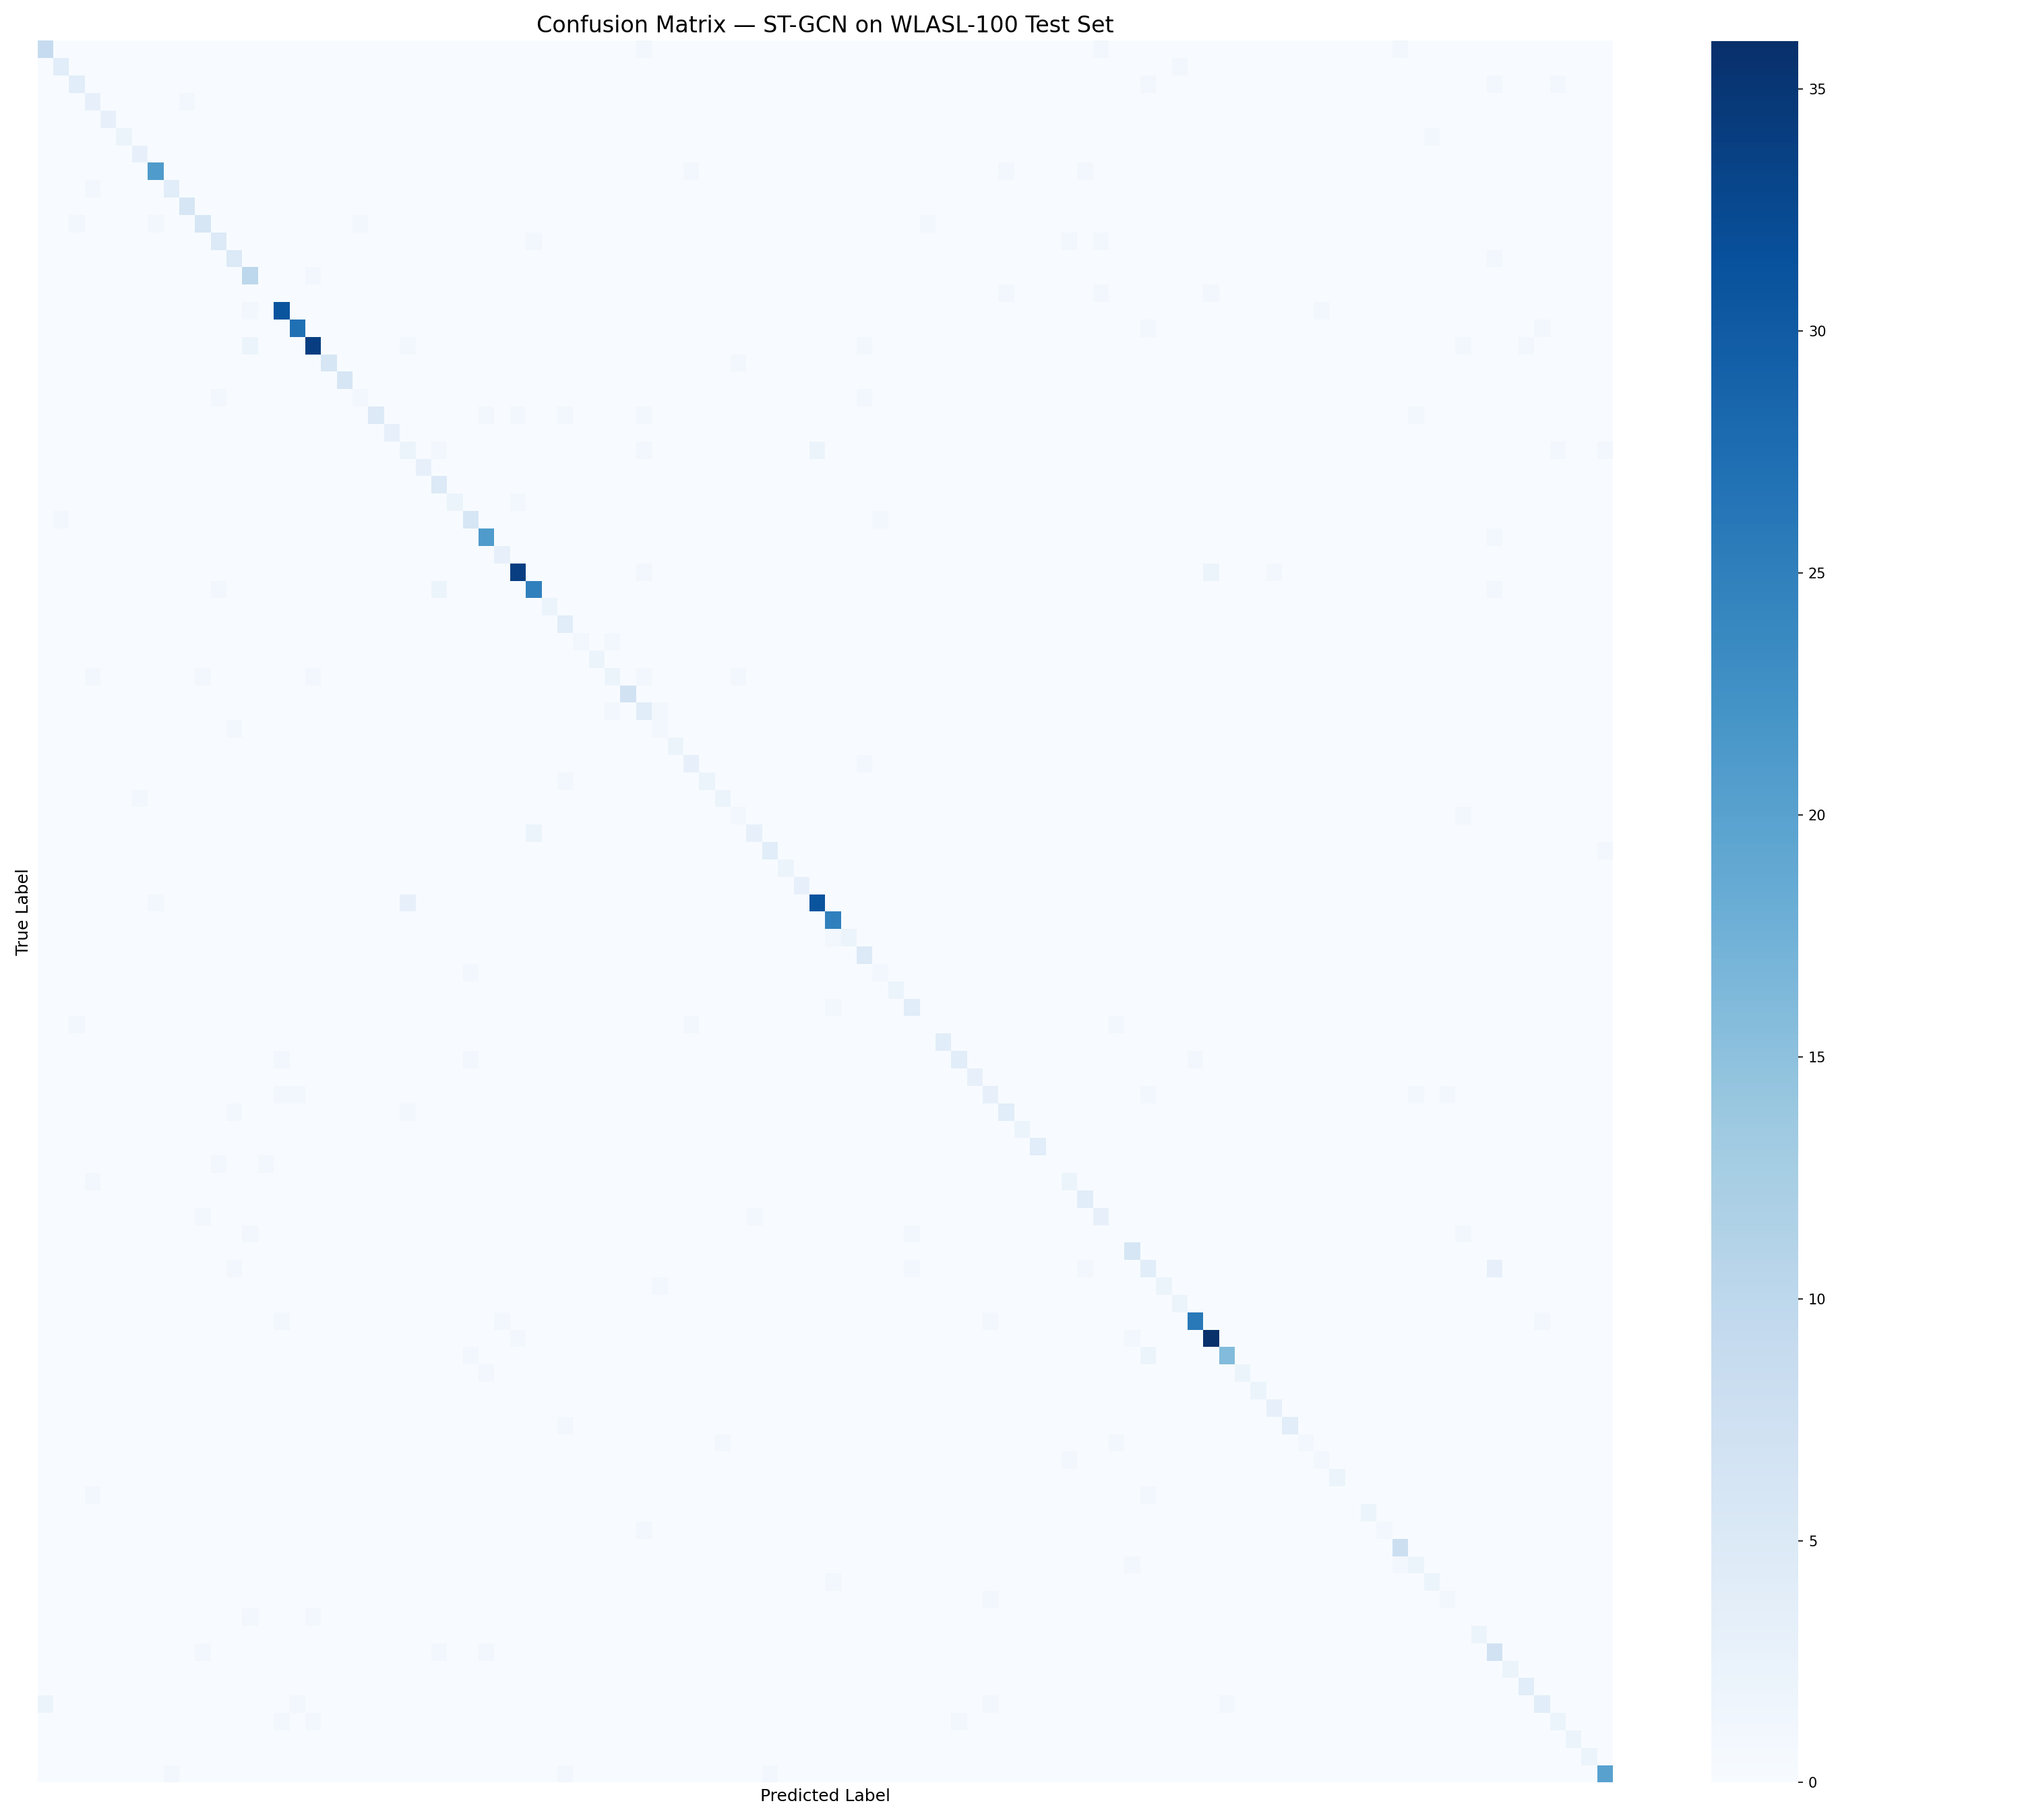
\includegraphics[height=0.6\textheight]{src/confusion_matrix.png}
        \caption{Confusion matrix (100 classes)}
    \end{figure}
\end{frame}

\begin{frame}{Conclusion}
    \begin{itemize}
        \item Successfully built a real-time WSLR system.
        \item ST-GCN with an adaptive graph delivers superior performance.
        \item A Top-5 accuracy of 88.0\% indicates readiness for practical deployment.
    \end{itemize}
\end{frame}

% ==========================================================================
% ====================  IN-DEPTH EXTENDED MATERIAL (ADDED)  =================
% ==========================================================================

\begin{frame}
    \centering
    {\usebeamercolor[fg]{title}\Large \textbf{In-Depth Extended Material}}\\[0.35cm]
    \normalsize From State-of-the-Art Architectures to Low-Latency Systems Optimization\\[0.2cm]
    \footnotesize\textit{(Reference material for in-depth discussion)}
\end{frame}

% ==========================================
\section{4. State-of-the-Art Directions: Beyond ST-GCN}
% ==========================================
\begin{frame}{The Core Bottleneck of ST-GCN}
    \begin{alertblock}{Limitations of a Static Adjacency Matrix}
        ST-GCN fixes the graph structure according to \textbf{human anatomy}.
    \end{alertblock}
    \vspace{0.4cm}
    \begin{itemize}
        \item Connections between joints are hard-coded in advance.
        \item It cannot learn \textbf{flexible cross-links} among the hands, face, and body.
        \item Semantic cues are lost when a sign requires coordinating anatomically distant parts.
    \end{itemize}
    \vspace{0.3cm}
    \centering\textit{$\Rightarrow$ Dynamic and multi-modal architectures are required to reach SOTA.}
\end{frame}

\begin{frame}{Four Directions Beyond ST-GCN}
    \begin{enumerate}
        \item \textbf{Multi-cue fusion} -- combining multiple data streams.
        \vspace{0.2cm}
        \item \textbf{VAC} -- a temporal alignment constraint.
        \vspace{0.2cm}
        \item \textbf{Gloss-free (VLM)} -- learning without intermediate labels.
        \vspace{0.2cm}
        \item \textbf{CTR-GCN} -- dynamic graphs per feature channel.
    \end{enumerate}
    \vspace{0.4cm}
    \centering\small\textit{The following slides examine each direction in turn.}
\end{frame}

\begin{frame}{Direction 1 -- Multi-cue Fusion}
    \begin{block}{Ingesting Multiple Streams in Parallel}
        \begin{itemize}
            \item \textbf{Skeleton:} hand shape and trajectory.
            \item \textbf{Raw RGB:} mouth shape and facial-expression cues.
            \item \textbf{Optical flow:} fine-grained motion direction.
        \end{itemize}
    \end{block}
    \vspace{0.3cm}
    \begin{itemize}
        \item Each stream compensates for the blind spots of the others.
        \item The key issue is \textbf{how the streams are fused} (see next slide).
    \end{itemize}
\end{frame}

\begin{frame}{Direction 1 -- The Cross-Attention Mechanism}
    \begin{columns}[T]
        \begin{column}{0.52\textwidth}
            \begin{block}{Late vs. Early/Intermediate Fusion}
                Modern models fuse \emph{early/intermediately} via cross-attention, rather than merging at the final layer (late fusion).
            \end{block}
            \vspace{0.2cm}
            \begin{itemize}
                \item $Q \leftarrow$ the \textbf{RGB} stream
                \item $K,\,V \leftarrow$ the \textbf{pose} stream
            \end{itemize}
        \end{column}
        \begin{column}{0.44\textwidth}
            \begin{exampleblock}{Attention formula}
                \[
                    \mathrm{Attn}(Q,K,V)=\mathrm{softmax}\!\left(\frac{QK^{\top}}{\sqrt{d_k}}\right)V
                \]
            \end{exampleblock}
            \vspace{0.1cm}
            \centering\small\textit{The model learns autonomously ``when to attend to the face and when to attend to the fingers''.}
        \end{column}
    \end{columns}
\end{frame}

\begin{frame}{Direction 2 -- VAC (Visual Alignment Constraint)}
    \begin{alertblock}{Weakness of the Conventional CTC Loss}
        It maps a 100-frame video to 3 glosses without specifying which gloss occurs at which frame $\Rightarrow$ the network becomes ``lazy'' and yields blurred features.
    \end{alertblock}
    \vspace{0.3cm}
    \begin{block}{How VAC Addresses This}
        \begin{itemize}
            \item Forces the model to produce a sharper \textbf{pseudo-alignment}.
            \item Encourages features of adjacent frames to cluster into distinct semantic groups.
            \item Adds auxiliary loss terms that assist backpropagation.
        \end{itemize}
    \end{block}
\end{frame}

\begin{frame}{Direction 3 -- Gloss-Free via VLMs}
    \begin{block}{Joint Embedding Space (CLIP-style)}
        Contrastive learning pulls the embedding of a \emph{signing video} close to that of its corresponding \emph{text sentence} in a high-dimensional space.
    \end{block}
    \vspace{0.3cm}
    \begin{exampleblock}{Benefits}
        \begin{itemize}
            \item Eliminates the intermediate gloss-annotation stage entirely.
            \item Saves annotation costs of up to millions of dollars on large datasets.
        \end{itemize}
    \end{exampleblock}
\end{frame}

\begin{frame}{Direction 4 -- Dynamic Graphs (CTR-GCN)}
    \begin{block}{From a Static to a Per-Channel Dynamic Adjacency}
        Instead of a single anatomically fixed adjacency matrix $A$, CTR-GCN \textbf{learns parameters} that generate distinct graph connections for \emph{each feature channel}.
    \end{block}
    \vspace{0.3cm}
    \begin{itemize}
        \item Each channel may carry a different graph topology.
        \item The left hand may \textbf{connect directly} to the right eye if that link is semantically meaningful.
    \end{itemize}
\end{frame}

% ==========================================
\section{5. The Real-Time Systems Problem}
% ==========================================
\begin{frame}{The Time-Budget Constraint (30 FPS)}
    \begin{alertblock}{The Physical Law of Real-Time Processing}
        At 30 FPS, each frame has only $\mathbf{33.3\,ms}$. Exceeding this budget $\Rightarrow$ frame drops and loss of motion data.
    \end{alertblock}
    \vspace{0.4cm}
    \begin{center}
    \resizebox{\textwidth}{!}{%
    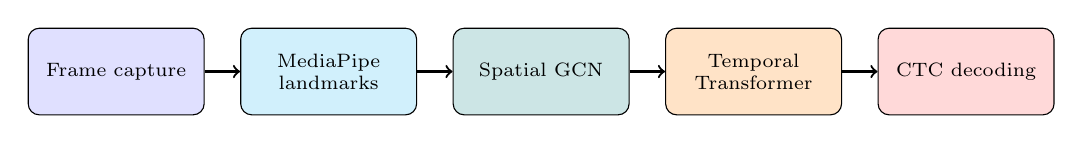
\begin{tikzpicture}[
        node distance=0.45cm,
        stage/.style={draw, rounded corners, minimum height=1.1cm, text width=2cm, align=center, font=\scriptsize}
    ]
        \node[stage, fill=blue!12]               (n1) {Frame capture};
        \node[stage, fill=cyan!18,  right=of n1] (n2) {MediaPipe landmarks};
        \node[stage, fill=teal!20,  right=of n2] (n3) {Spatial GCN};
        \node[stage, fill=orange!22,right=of n3] (n4) {Temporal Transformer};
        \node[stage, fill=red!15,   right=of n4] (n5) {CTC decoding};
        \draw[->, thick] (n1) -- (n2);
        \draw[->, thick] (n2) -- (n3);
        \draw[->, thick] (n3) -- (n4);
        \draw[->, thick] (n4) -- (n5);
    \end{tikzpicture}}
    \end{center}
    \vspace{0.3cm}
    \centering\small All five pipeline stages must fit within the $33.3\,ms$ budget.
\end{frame}

\begin{frame}{Challenge 1 -- Transformer Cache Locality}
    \begin{block}{Self-Attention Has $\mathcal{O}(N^2)$ Complexity}
        A long sliding window ($\sim$200 frames) produces enormous matrices.
    \end{block}
    \vspace{0.3cm}
    \begin{itemize}
        \item Matrices repeatedly overflow the L1/L2 cache (cache thrashing).
        \item Data is evicted to VRAM, or worse, to system RAM.
        \item Access speed can degrade by a factor of thousands.
    \end{itemize}
\end{frame}

\begin{frame}{Challenge 2 -- Input Bandwidth Optimization}
    \begin{alertblock}{The Conventional Copy Path (Slow)}
        Camera $\to$ Kernel Space $\to$ User Space $\to$ PCIe $\to$ VRAM.
    \end{alertblock}
    \vspace{0.3cm}
    \begin{exampleblock}{Kernel Bypass / Zero-Copy (GPUDirect)}
        \begin{itemize}
            \item Writes the video stream \textbf{directly} into GPU VRAM.
            \item Bypasses the CPU and operating system entirely.
            \item Maximizes throughput, achieving microsecond-level latency.
        \end{itemize}
    \end{exampleblock}
\end{frame}

% ==========================================
\section{6. The Commercial Landscape}
% ==========================================
\begin{frame}{Lesson 1 -- The Smart-Glove ``Graveyard''}
    \begin{alertblock}{Why Did Smart Gloves Fail?}
        Wearable-sensor solutions suffer from numerous physical limitations.
    \end{alertblock}
    \vspace{0.3cm}
    \begin{itemize}
        \item Flex sensors are limited in their degrees of freedom (DoF).
        \item IMUs suffer from sensor drift when one hand occludes the other.
        \item They \textbf{ignore} the upper body and facial expression entirely -- which carry substantial meaning.
    \end{itemize}
\end{frame}

\begin{frame}{Lesson 2 -- The Core Infrastructure: Google MediaPipe}
    \begin{block}{A Graph-Based Architecture Behind $\sim$90\% of Real-Time Applications}
        The computation pipeline is divided into independent ``nodes''.
    \end{block}
    \vspace{0.3cm}
    \begin{itemize}
        \item The hand-detection and eye-tracking nodes run independently and multi-threaded.
        \item They share \textbf{pre-allocated} tensors.
        \item This avoids garbage-collection latency within the real-time loop.
    \end{itemize}
\end{frame}

\begin{frame}{Lesson 3 -- Domain Shift: B2C vs. B2B}
    \begin{columns}[T]
        \begin{column}{0.5\textwidth}
            \begin{alertblock}{Mobile Applications (B2C)}
                \begin{itemize}
                    \item Shaky camera angles and backlighting.
                    \item Complex backgrounds corrupt the feature vectors.
                    \item Prone to failure due to domain shift.
                \end{itemize}
            \end{alertblock}
        \end{column}
        \begin{column}{0.5\textwidth}
            \begin{exampleblock}{Fixed Stations (B2B) -- SignAll}
                \begin{itemize}
                    \item Installed in schools and hospitals.
                    \item Fixed cameras and standardized lighting.
                    \item Reduces environmental error.
                \end{itemize}
            \end{exampleblock}
        \end{column}
    \end{columns}
\end{frame}

% ==========================================
\section{7. Deployment Optimization: ONNX Runtime \& C++}
% ==========================================
\begin{frame}{Why Abandon Python in Production?}
    \begin{alertblock}{Limitations of Native Python}
        \begin{itemize}
            \item The \textbf{GIL} (Global Interpreter Lock) prevents true multi-threading.
            \item Large overhead from dynamic type checking.
        \end{itemize}
    \end{alertblock}
    \vspace{0.3cm}
    \begin{exampleblock}{Solution: ONNX + C/C++ with Memory Pooling}
        \begin{itemize}
            \item Avoid calling \texttt{malloc}/\texttt{new} inside the inference loop (which causes tail latency).
            \item Allocate one large RAM block at start-up and reuse it for every frame.
        \end{itemize}
    \end{exampleblock}
\end{frame}

\begin{frame}{The Three Graph-Optimization Levels of ONNX Runtime}
    \begin{block}{Level 1 -- Constant Folding}
        Pre-computes operations between constants once at load time $\Rightarrow$ fewer nodes to process.
    \end{block}
    \begin{block}{Level 2 -- Layer Fusion}
        Fuses Conv $\to$ BN $\to$ ReLU into a single \textbf{megakernel}; data stays in registers and is written to VRAM only once.
    \end{block}
    \begin{block}{Level 3 -- Hardware Execution Provider}
        Recompiles using native hardware APIs, e.g.\ \textbf{DirectML} (DirectX 12) for any GPU.
    \end{block}
\end{frame}

\begin{frame}{The Mathematics of Layer Fusion}
    \begin{columns}[T]
        \begin{column}{0.46\textwidth}
            \textbf{Before fusion:}
            \begin{align*}
                \text{Conv:}\quad & y = Wx + b \\[0.25cm]
                \text{BN:}\quad & z = \gamma\,\frac{y-\mu}{\sqrt{\sigma^2+\epsilon}} + \beta
            \end{align*}
            \vspace{0.2cm}
            \begin{block}{Idea}
                \small A linear-algebraic transformation performed \emph{prior} to inference.
            \end{block}
        \end{column}
        \begin{column}{0.52\textwidth}
            \textbf{After fusion (re-parameterized weights):}
            \[ W_{\text{fused}} = \frac{\gamma\cdot W}{\sqrt{\sigma^2+\epsilon}} \]
            \[ b_{\text{fused}} = \frac{\gamma\cdot(b-\mu)}{\sqrt{\sigma^2+\epsilon}} + \beta \]
            \vspace{0.15cm}
            \begin{exampleblock}{Consequence}
                \small The BN layer is removed from the inference graph; millions of FLOPs are eliminated with error below $0.001\%$.
            \end{exampleblock}
        \end{column}
    \end{columns}
\end{frame}

\begin{frame}{Summary of the Extended Material}
    \begin{itemize}
        \item \textbf{Research:} Multi-cue + cross-attention, VAC, gloss-free (VLM), and CTR-GCN move beyond ST-GCN.
        \vspace{0.2cm}
        \item \textbf{Systems:} The $33.3\,ms$ budget, Transformer cache locality, and kernel bypass determine real-time feasibility.
        \vspace{0.2cm}
        \item \textbf{Deployment:} ONNX Runtime + C++ (memory pooling, layer fusion) turn SOTA papers into products running smoothly at 30 FPS.
    \end{itemize}
\end{frame}

% ==========================================================================
% ====================  END OF EXTENDED MATERIAL  ==========================
% ==========================================================================

\begin{frame}
    \centering
    \Huge \textbf{Thank you for your attention!}
\end{frame}

\end{document}